% AeroCast-AI -- Phase 1 report (IEEE conference format, short version).
% Build: cd report && tectonic -X compile main.tex   (or: pdflatex main && bibtex main && pdflatex main && pdflatex main)
% figures/ and tables/ are generated by scripts/export_report_assets.py from results/ (never edit by hand).
% The prose is hand-written; scripts/check_report_numbers.py asserts the quoted numbers against results/.
% The earlier 22-page version is kept locally in report/long_version/ (git-ignored).
\documentclass[conference]{IEEEtran}
\usepackage[T1]{fontenc}
\usepackage{cite}
\usepackage{amsmath,amssymb}
\usepackage{graphicx}
\usepackage{booktabs}
\usepackage{array}
\usepackage[inline]{enumitem}
\usepackage[hidelinks]{hyperref}
\graphicspath{{figures/}}
\setlist[itemize]{leftmargin=1.1em,itemsep=1pt,topsep=2pt,parsep=0pt}
\newcommand{\tabsize}{\footnotesize}

\begin{document}

\title{Day-Ahead Flight Delay Risk for NYC Departures:\\
Leakage-Aware Learning and Calibration under Seasonal Shift}

\author{\IEEEauthorblockN{Nipun Patlori, Anushka Tyagi, Mohan Kumar C R, Omkar Hadole, Krish Dabas}
\IEEEauthorblockA{Team T49 --- Advanced Machine Learning, Semester 5 --- Project 21, Phase 1 (machine learning)}}

\maketitle

\begin{abstract}
We predict, at \textbf{20:00 on the evening before departure}, whether a flight leaving New York (EWR, JFK, LGA; 2013) will arrive at least 15 minutes late. The study is built around this decision clock: every feature, training label, calibration label and threshold must be known by then. Three automated leakage tests enforce the clock, and one of them found a same-day leak in two aircraft-rotation features, which we removed. Regularised logistic regression and XGBoost use 43 schedule, congestion, calendar and past-delay features, and are compared with a base-rate prior and a route-history heuristic under a chronological split with rolling-origin cross-validation. Logistic regression is selected by cross-validation (PR-AUC 0.471 vs 0.450). On the Nov--Dec test window it reaches \textbf{PR-AUC 0.393}, against 0.407 for XGBoost, 0.353 for route history and 0.258 for the prior; the two learned models are not statistically distinguished. Flagging the riskiest 10\% of flights each day gives \textbf{precision 0.448, 1.73 times the base rate}. A calibrator fitted on the calm autumn months \textbf{fails in December} (ECE 0.143), while a causal rolling recalibration keeps test ECE at 0.027.
\end{abstract}

\begin{IEEEkeywords}
flight delay prediction, data leakage, gradient boosting, probability calibration, temporal validation
\end{IEEEkeywords}

%====================================================================
\section{Introduction}\label{sec:intro}
Flight delays cascade: a late aircraft or a congested departure bank turns one disruption into many. Remedies such as adding buffer, swapping an aircraft or re-timing a flight take time, so operators need to know \emph{the evening before} which flights are most at risk.
\begin{itemize}
\item \textbf{Task.} For each flight scheduled to leave EWR, JFK or LGA on day $D$, estimate $P(\text{arrival delay}\ge15\text{ min})$ at 20:00 New York time on $D-1$, and rank the day's flights by it.
\item \textbf{Why a decision clock.} Every past outcome sits in the same table, so a careless join or rolling window silently uses information that would not exist at prediction time. A score obtained that way answers a question no operator can ask.
\item \textbf{Why calibrated probabilities.} A review desk that works down a ranked list needs only the order; a desk that sets a probability threshold or budgets buffer time needs probabilities that mean what they say. We evaluate both.
\end{itemize}

\textbf{Contributions.}
\begin{itemize}
\item A \textbf{decision clock} applied to features, training, cross-validation, calibration and thresholds, enforced by three leakage tests; one test exposed a real leak, which was removed (Sec.~\ref{sec:clock}).
\item A \textbf{controlled comparison} of logistic regression and XGBoost against two reference models, with the final model fixed by a rule declared before testing.
\item A study of \textbf{calibration under seasonal shift}: a static recalibrator and a causal rolling alternative.
\item A \textbf{daily review-desk analysis} of how well the ranking concentrates delayed flights.
\end{itemize}
\textbf{Scope.} This is Phase~1 (machine learning) of Project~21, \emph{Flight Delay Prediction and Rescheduling}. A compact MLP with learned airline and airport embeddings is planned for the next phase and will reuse the same clock, features and splits.

%====================================================================
\section{Background and Related Work}\label{sec:related}
\begin{itemize}
\item \textbf{Leakage.} Kaufman et al.~\cite{kaufman2012leakage} define leakage as the use of information about the target that would not legitimately be available at prediction time, and propose avoiding it by a strict \emph{learn--predict separation} that marks which data are legitimately available for each prediction. Our decision clock applies this rule to a daily forecasting problem, through an availability date attached to every outcome.
\item \textbf{Calibration.} Guo et al.~\cite{guo2017calibration} show that modern neural networks, although accurate, are often over-confident, measure this with the expected calibration error (ECE) and reliability diagrams, and fix it after training with a one-parameter version of Platt scaling. Their evaluation assumes the test data resemble the calibration data; we test what happens when the season changes.
\item \textbf{Gap.} We combine both concerns in one day-ahead pipeline: strict outcome availability for every feature, label and fitting step, and probability quality when the season changes, with a fair comparison of a linear and a boosted model.
\end{itemize}

%====================================================================
\section{Data and Exploratory Analysis}\label{sec:data}
\begin{itemize}
\item \textbf{Source.} The Kaggle Flights dataset\footnote{\url{https://www.kaggle.com/datasets/mahoora00135/flights}, derived from the \texttt{nycflights13} R package.}: 336{,}776 departures from EWR, JFK and LGA in 2013, with carrier, flight and tail number, route, distance, schedule and recorded outcomes.
\item \textbf{Quality.} No duplicate flights. Missing values are structural: 8{,}255 flights have no departure time (cancelled) and 1{,}175 departed without an arrival delay (diverted). All 2{,}512 missing tail numbers belong to cancelled flights, a fact that matters for leakage (Sec.~\ref{sec:leak}).
\item \textbf{Target.} $y=\mathbb{1}[\text{arrival delay}\ge15\text{ min}]$, the U.S. Bureau of Transportation Statistics on-time convention; 24.5\% of completed flights are late. Cancelled and diverted flights have no arrival delay and are excluded from the label, but remain in the schedule-based congestion counts, because a cancellation is not known the evening before. A sensitivity analysis counts them as delayed.
\end{itemize}

\begin{figure*}[!t]
\centering
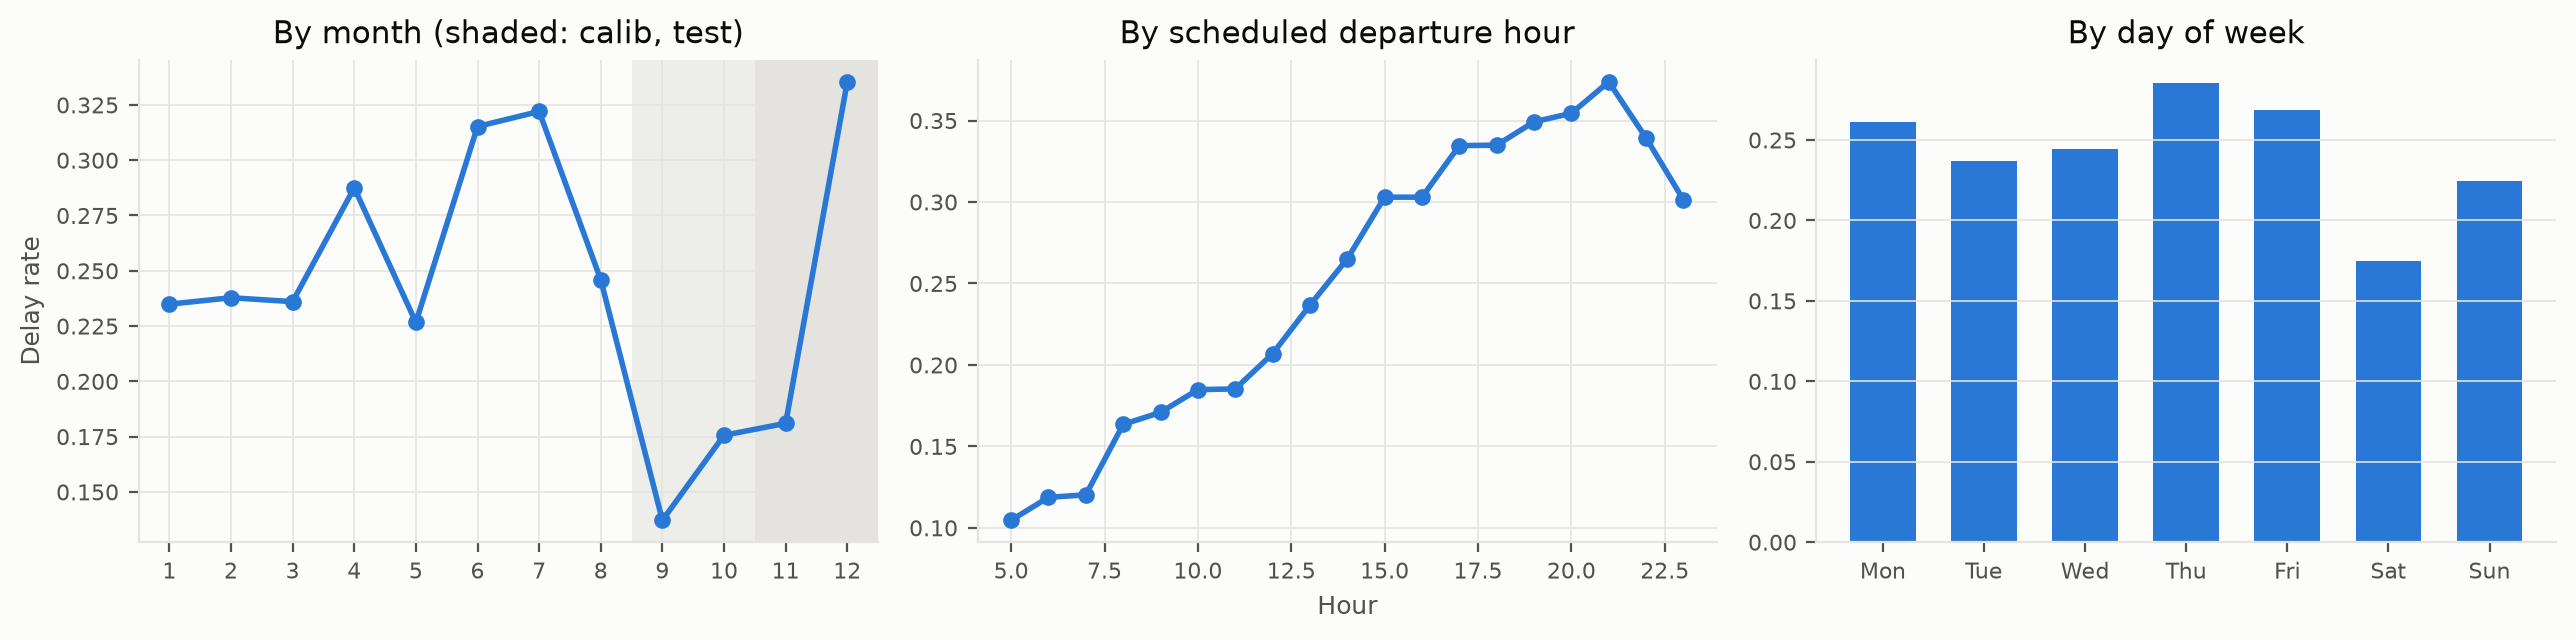
\includegraphics[width=0.86\textwidth]{eda_rate_by_time.png}
\caption{Delay rate by month (shaded: calibration and test windows), scheduled departure hour and weekday.}
\label{fig:eda}
\end{figure*}

\textbf{Patterns that drive the design} (Fig.~\ref{fig:eda}):
\begin{itemize}
\item \textbf{Time of day.} The late rate rises from 10.5\% at 05:00 to 37.4\% at 21:00 as delays propagate through the day $\Rightarrow$ cyclic time-of-day features.
\item \textbf{Season.} Monthly rates range from 13.7\% (September) to 33.5\% (December). The calm autumn followed by an extreme December makes a chronological split a natural stress test for calibration.
\item \textbf{Short memory.} The daily delay rate has lag-1 autocorrelation 0.40, so yesterday's disruption is informative $\Rightarrow$ day-level history features.
\item \textbf{Congestion.} Busy departure banks cluster in the evening, when delays are high anyway, so the raw association is confounded with the hour. Comparing banks \emph{within} each hour removes this: the busiest third is still 4.5 percentage points more often late than the quietest, and later in 13 of 16 hours (Fig.~\ref{fig:cong}) $\Rightarrow$ scheduled-congestion counts.
\end{itemize}

\begin{figure}[!t]
\centering
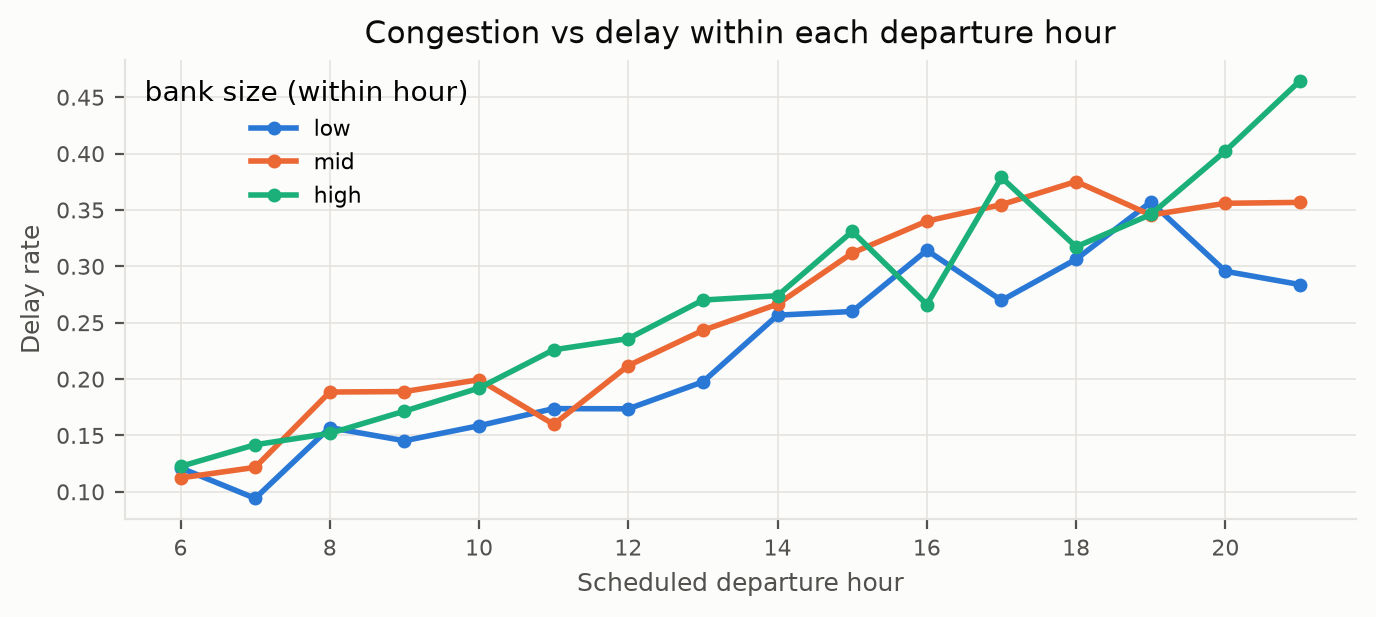
\includegraphics[width=\columnwidth]{eda_congestion_within_hour.png}
\caption{Delay rate by scheduled-bank size (terciles within each hour), holding the departure hour fixed.}
\label{fig:cong}
\end{figure}

%====================================================================
\section{Decision Clock and Leakage}\label{sec:clock}
\begin{itemize}
\item \textbf{Clock.} Predictions for all flights of day $D$ are made at 20:00 New York time on $D-1$.
\item \textbf{When is an outcome known?} An arrival delay becomes known at the actual gate arrival, converted to New York time with a fixed destination time-zone table and the 2013 daylight-saving rule; a cancellation is assumed known at the scheduled departure.
\item \textbf{Availability date.} An outcome known at time $t$ may first be used for target day
\end{itemize}
\[
a(t)=\lceil t-20\,\mathrm{h}\rceil_{\text{day}}+1\text{ day}.
\]
History windows roll over availability dates, not flight dates. A flight on $D-1$ that lands at 22:30 has $a(t)=D+1$, so it cannot inform day $D$. This matters: 31.1\% of $D-1$ arrivals land after 20:00, and they are late 38.1\% of the time, against 18.3\% for earlier arrivals.

\begin{itemize}
\item \textbf{The clock also governs fitting.} Each cross-validation (CV) fold trains only on labels available at its first validation day. The final models use training labels available by 20:00 on 31~August (167 late-August outcomes are excluded), and the calibrator and threshold use Sep--Oct labels available by 31~October (251 excluded).
\item \textbf{How much would a later clock help?} Moving the cutoff to midnight raises the CV PR-AUC of logistic regression from 0.471 to 0.481: a gain of 0.010 that would come entirely from information an operator does not have at 20:00. A two-day lag (00:00 on $D-1$) lowers it to 0.459.
\end{itemize}

\subsection{Leakage tests}\label{sec:leak}
\begin{itemize}
\item \textbf{(a) Future outcomes.} Replace every post-departure value from 15~June onward with random numbers and rebuild all features. Features up to and including 15~June must be identical: \textbf{0} cells change, while 4{,}558{,}344 cells after the cutoff do change, so the test can fail.
\item \textbf{(b) Late evening arrivals.} Randomise the outcomes of $D-1$ flights that landed after 20:00: \textbf{0} feature cells of day $D$ change (tested on 14~Feb, 11~Jul and 20~Dec). Randomising the flights that landed before 20:00 changes about 12{,}000--13{,}000 cells, which confirms the test is sensitive.
\item \textbf{(c) Same-day cancellations.} Cancel 30\% of a day's flights the way the raw data records it (times and tail number blanked) and rebuild: \textbf{0} features of the day's other flights may change.
\end{itemize}

\textbf{A leak found and removed.} An earlier version had two \emph{aircraft-rotation} features: the aircraft's leg number that day and its number of NYC departures, both counted by tail number. Because cancelled flights lose their tail number, test~(c) showed that a cancellation on day $D$ changed these features for the aircraft's other day-$D$ flights. For example, an aircraft planned to leave at 09:29, 14:50 and 21:40 on 10~Oct: cancelling the 14:50 leg turned the 21:40 flight from ``leg 3 of 3'' into ``leg 2 of 2'', although the plan known at 20:00 on 9~Oct still had three legs. Both features were removed on leakage grounds (45~$\to$~43 features); the CV PR-AUC of logistic regression changed by less than 0.001.

%====================================================================
\section{Features}\label{sec:features}
The 43 features fall into five groups (Table~\ref{tab:features}). Time of day and weekday are encoded as sine/cosine pairs so that 23:59 and 00:01 are neighbours. Congestion counts \emph{scheduled} flights, including ones that will later be cancelled, because cancellations are unknown the evening before.

\begin{table}[!t]
\caption{Feature groups ($n$ = number of features).}
\label{tab:features}
\centering\tabsize
% generated by scripts/export_report_assets.py from results/ -- do not edit
% needs \usepackage{booktabs}
\begin{tabular}{@{}lrp{5.3cm}@{}}
\toprule
Group & $n$ & Content \\
\midrule
Identifiers & 3 & carrier, origin, destination \\
Schedule & 10 & cyclic departure and arrival time of day, cyclic weekday, departure hour, weekend flag, days to holiday (cap 14), log distance \\
Congestion & 5 & scheduled flights at the origin in the hour, the $\pm$1 h window and the day; destination and carrier daily volumes \\
Entity history & 18 & smoothed delay rate and log-volume of origin (7 d), carrier (7, 14 d), destination, route, carrier-route, origin-hour, flight number and tail number (14 d) \\
Day history & 7 & network delay rate (1, 7 d); origin delay rate, volume and mean delay (1 d); network and origin cancellation rates (1 d) \\
\bottomrule
\end{tabular}

\end{table}

\begin{figure}[!t]
\centering
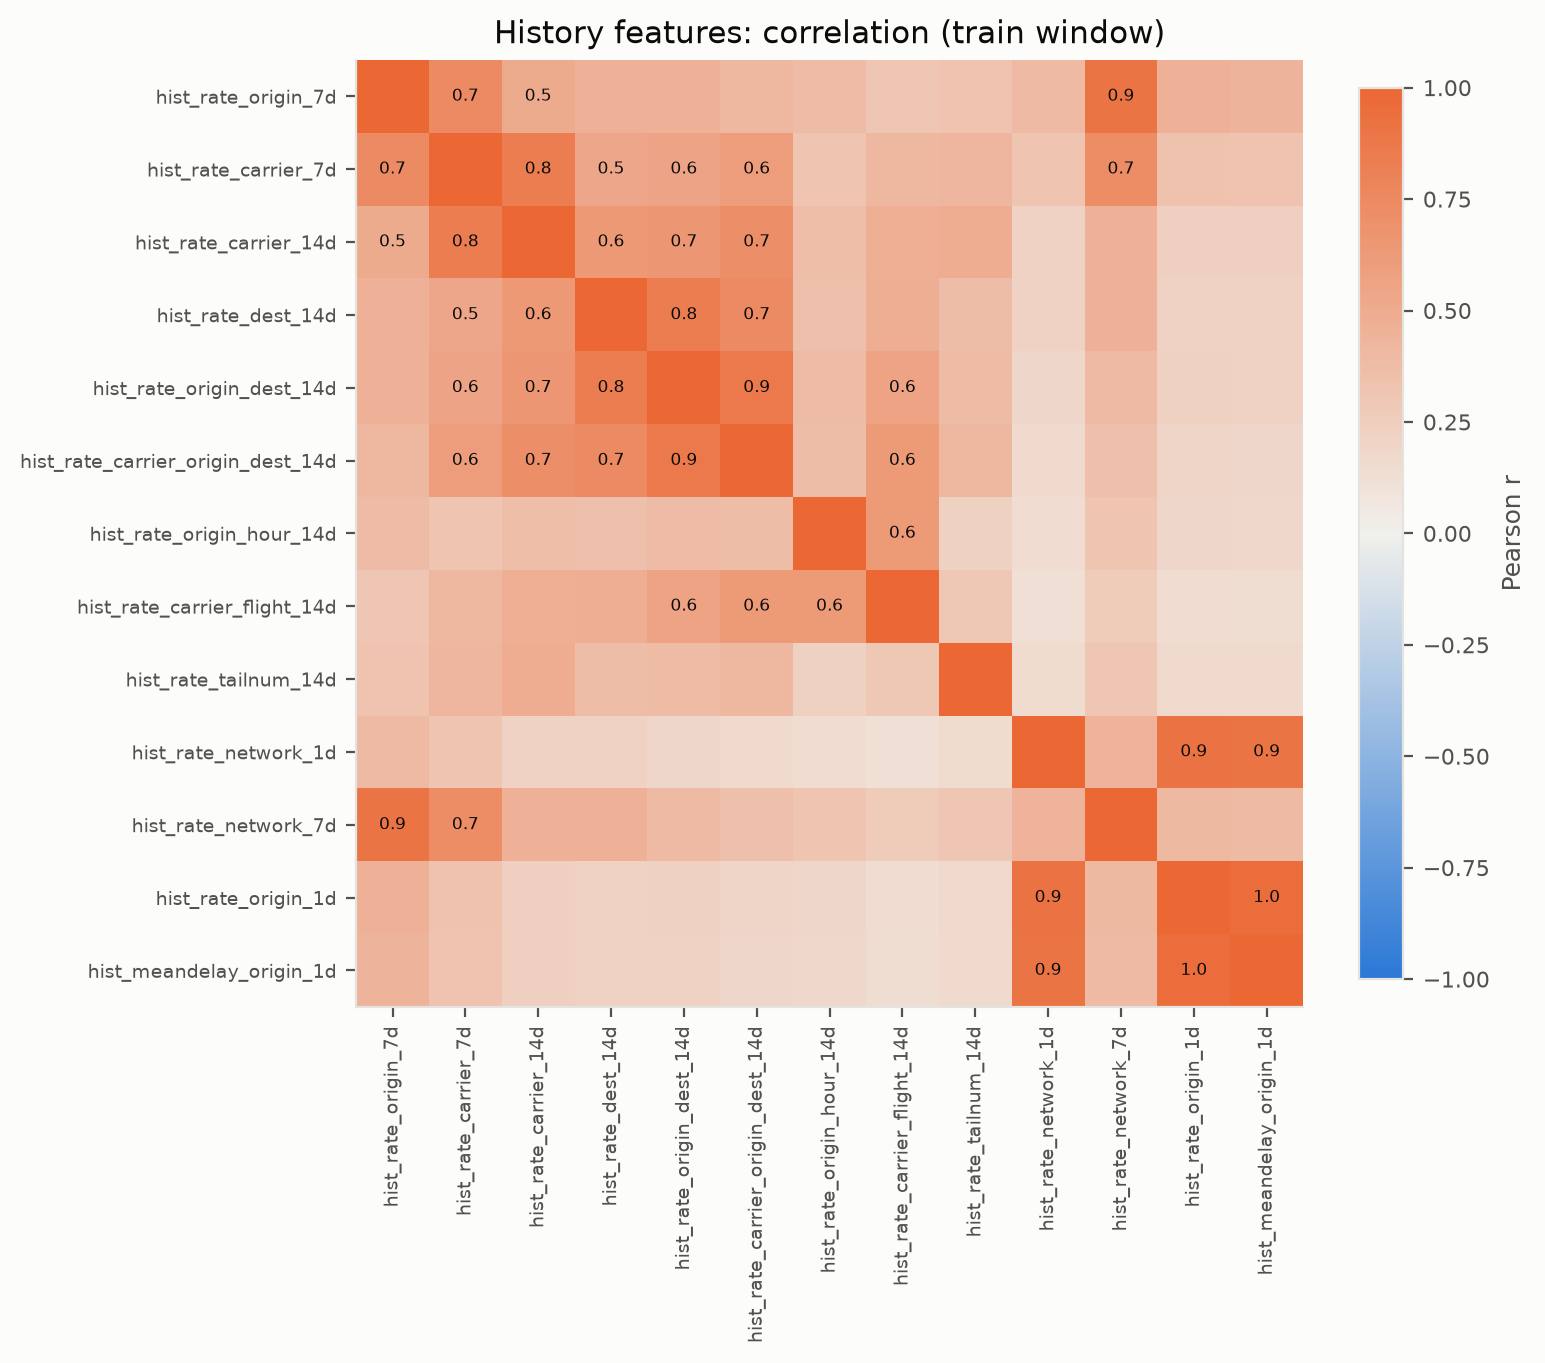
\includegraphics[width=0.95\columnwidth]{eda_history_corr_heatmap.png}
\caption{Correlation of the history features on the training window.}
\label{fig:corr}
\end{figure}

\textbf{Shrunk history rates.} A tail number seen once and late has an empirical late rate of 100\%. Entity rates are therefore shrunk towards the network rate $\pi_D$ of the previous 28 days (beta-binomial posterior mean):
\[
\hat r_{k,D}=\frac{\text{late}_k+m\,\pi_D}{\text{flights}_k+m},
\]
where the counts cover outcomes available for $D$ within the window. This is the posterior mean of the entity's late probability under a $\mathrm{Beta}(m\pi_D,\,m(1-\pi_D))$ prior: $m$ acts as a number of pseudo-flights at the network rate. With one late flight on a thin route and $\pi_D=0.247$, $m=5$ gives $(1+5\times0.247)/6=0.372$ instead of 1.0.
\begin{itemize}
\item \textbf{Correlated history rates.} Nested windows on the same key, and network and origin rates that move together, are strongly correlated, some at $|r|$ close to 1 (Fig.~\ref{fig:corr}). Hence logistic regression is L2-regularised, and importance is measured per group, not per feature.
\item \textbf{Tuning.} The shrinkage $m\in\{5,20,50\}$ and the long window $w\in\{14,28,56\}$ days were tuned jointly with the logistic-regression penalty by rolling CV: $m=5$, $w=14$ days, $C=0.1$.
\item \textbf{No month feature.} Training sees only January--August, so September--December month values never occur in training. Adding cyclic month features lowers the CV PR-AUC of logistic regression from 0.471 to 0.469; recent history already tracks the season.
\end{itemize}

%====================================================================
\section{Models and Calibration}\label{sec:models}
\subsection{Logistic regression}
$P(y=1\mid x)=\sigma(w^\top x+b)$, fitted by minimising the L2-regularised log-loss
\[
\mathcal{L}(w)=-\tfrac1n\textstyle\sum_i\big[y_i\log p_i+(1-y_i)\log(1-p_i)\big]+\tfrac{1}{2Cn}\lVert w\rVert^2 .
\]
\begin{itemize}
\item \textbf{Why regularise.} Correlated history rates make unpenalised coefficients unstable. The L2 penalty is the maximum-a-posteriori estimate under a zero-mean Gaussian prior on $w$; smaller $C$ shrinks harder. $C$ was chosen from $\{0.0003,\dots,1\}$ by rolling CV; the curve is flat above $C\approx0.003$.
\item \textbf{Why log-loss.} Log-loss (and the Brier score) are \emph{proper} scoring rules: their expected value is minimised only by the true probability, so training with log-loss pushes towards calibrated probabilities on the training distribution. ECE is not a proper score and depends on the binning, so it is reported alongside the Brier score, not instead of it.
\item \textbf{Preprocessing.} Identifiers are one-hot encoded (categories with fewer than 50 flights merged); numeric features are median-imputed with missing-value indicators and standardised, all fitted on the training labels only.
\end{itemize}

\subsection{XGBoost}
An additive ensemble of regression trees. Tree $t$ minimises a second-order Taylor approximation of the log-loss plus a complexity penalty,
\[
\tilde{\mathcal L}^{(t)}=\textstyle\sum_i\big[g_if_t(x_i)+\tfrac12h_if_t(x_i)^2\big]+\gamma J_t+\tfrac12\lambda\lVert v_t\rVert^2 ,
\]
with $g_i=p_i-y_i$ and $h_i=p_i(1-p_i)$, $J_t$ leaves and leaf weights $v_t$. The optimal leaf weight is $v_j^*=-G_j/(H_j+\lambda)$, and a split is kept when its gain
\[
\tfrac12\Big[\tfrac{G_L^2}{H_L+\lambda}+\tfrac{G_R^2}{H_R+\lambda}-\tfrac{(G_L+G_R)^2}{H_L+H_R+\lambda}\Big]-\gamma
\]
is positive ($G$, $H$: sums of $g_i$, $h_i$ in a node).
\begin{itemize}
\item \textbf{Search.} 16 of 48 combinations of depth, minimum child weight, column subsample, $\lambda$ and learning rate, each with early stopping on the CV folds. Selected: depth 2, learning rate 0.1, minimum child weight 100, row and column subsample 0.8, $\lambda=10$, 108 trees.
\item \textbf{Inputs.} Native categorical splits and native missing-value handling; no one-hot encoding or imputation.
\end{itemize}

\subsection{Reference models}
The \textbf{prior} gives every flight the training base rate (no flight-specific information). \textbf{Route history} is the shrunk 14-day carrier-route late rate alone. A learned model must beat this transparent heuristic to justify itself.

\subsection{Calibration}
\begin{itemize}
\item \textbf{Platt scaling} maps a score $p$ to $\sigma(a\,\mathrm{logit}\,p+b)$; with $a>0$ it keeps the ranking. \textbf{Isotonic regression} fits any monotone step function.
\item \textbf{ECE}~\cite{guo2017calibration} averages the gap between observed rate and mean prediction over 15 equal-width probability bins $B_b$:
\end{itemize}
\[
\mathrm{ECE}=\textstyle\sum_b\frac{|B_b|}{n}\,\big|\bar y_b-\bar p_b\big| .
\]
\begin{itemize}
\item \textbf{Static rule} (declared before testing). Fit Platt and isotonic on September, compare ECE on October, and adopt the better one only if it lowers ECE by more than 0.005; then refit on Sep--Oct. Logistic regression over-predicts in the calm autumn and adopts Platt (October ECE gain 0.030); for XGBoost both recalibrators make October worse (gain $-0.020$), so it stays raw (Table~\ref{tab:calsel}).
\item \textbf{Why a static calibrator can fail.} By Bayes' rule, if only the base rate changes from $\pi$ to $\pi'$ (label shift), the correct probability changes by a constant on the logit scale: $\mathrm{logit}\,p'=\mathrm{logit}\,p+\mathrm{logit}\,\pi'-\mathrm{logit}\,\pi$. From the Sep--Oct base rate of 15.7\% to December's 33.5\%, this shift is about $+1.0$ logit, which a calibrator fitted once on Sep--Oct cannot know.
\item \textbf{Rolling Platt} (adaptive alternative). For each day $D$, refit Platt on the outcomes that became available in the previous 28 days and apply it to $D$'s flights. It uses the same availability dates as the features, so it never sees an unknown outcome, and its intercept follows the base rate with a lag.
\end{itemize}

\begin{table}[!t]
\caption{Static calibration rule: candidates fitted on September, checked on October. ECE gain: reduction in October ECE relative to raw scores.}
\label{tab:calsel}
\centering\tabsize
% generated by scripts/export_report_assets.py from results/ -- do not edit
% needs \usepackage{booktabs}
\begin{tabular}{llrrrr}
\toprule
Model & Calibrator & Oct ECE & Oct ECE (eq.-mass) & Oct Brier & ECE gain vs raw \\
\midrule
logreg & raw & 0.061 & 0.061 & 0.140 & 0.000 \\
logreg & platt & 0.035 & 0.035 & 0.138 & 0.026 \\
logreg & isotonic & 0.036 & 0.036 & 0.139 & 0.025 \\
xgboost & raw & 0.022 & 0.025 & 0.139 & 0.000 \\
xgboost & platt & 0.046 & 0.046 & 0.141 & -0.024 \\
xgboost & isotonic & 0.047 & 0.047 & 0.141 & -0.025 \\
\bottomrule
\end{tabular}

\end{table}

%====================================================================
\section{Evaluation Protocol}\label{sec:protocol}
\begin{itemize}
\item \textbf{Chronological split.} Training 8~Jan--31~Aug (211{,}684 flights, 26.5\% late; the first week is history warm-up), calibration Sep--Oct (55{,}628; 15.7\%), test Nov--Dec (53{,}991; 25.8\%, of which November 18.1\% and December 33.5\%).
\item \textbf{Rolling-origin CV} inside training: train on January to April and validate on May, then add May and validate on June, and so on to August. Each validation month lies strictly after its training data.
\item \textbf{Model-selection rule} (declared before testing). The family with the higher mean CV PR-AUC, each \emph{as deployed}: XGBoost with its fixed tree count, not the early-stopped score.
\item \textbf{Metrics.} PR-AUC as average precision, $AP=\sum_k(R_k-R_{k-1})P_k$, the main ranking metric: with one flight in four late, it reflects how pure the top of the ranking is, and its no-skill value is the base rate (ROC-AUC's is 0.5 at any base rate). Also ROC-AUC, the Brier score $\frac1n\sum_i(p_i-y_i)^2$, ECE, and lift, the policy precision divided by the base rate.
\item \textbf{Operating policies} (declared before testing). \emph{Primary:} a review desk flags the riskiest 10\% of each day's flights. \emph{Secondary:} a probability threshold frozen on Sep--Oct to reach precision $\ge0.40$; its test recall answers the brief's ``recall at an operational precision''.
\item \textbf{Uncertainty.} Flights on one day share weather and air-traffic shocks, so confidence intervals resample whole days (500 bootstrap replicates); model differences are paired on the same days.
\item \textbf{Disclosure.} Test metrics were seen several times during development. Every decision above rests on CV or Sep--Oct evidence, but the test results below should be read as exploratory, not as an untouched final check.
\end{itemize}

%====================================================================
\section{Results}\label{sec:results}
\subsection{Model selection (cross-validation)}
\begin{itemize}
\item \textbf{Logistic regression is selected} (Table~\ref{tab:cv}): CV PR-AUC 0.471 against 0.450 for XGBoost with its fixed tree count, 0.348 for route history and 0.278 for the prior.
\item \textbf{The margin is modest.} Logistic regression leads in three of four folds (paired differences $+0.003$, $+0.080$, $+0.005$, $-0.002$), and the fold-to-fold spread (SD about 0.07) is larger than the gap.
\item \textbf{An optimistic score avoided.} XGBoost's search score (0.475) early-stops on the very folds it is scored on; using it would have reversed the choice, so it is reported but not used.
\end{itemize}

\begin{table}[!t]
\caption{Rolling-CV PR-AUC on the validation months May--Aug.}
\label{tab:cv}
\centering\tabsize\setlength{\tabcolsep}{3.5pt}
% generated by scripts/export_report_assets.py from results/ -- do not edit
% needs \usepackage{booktabs}
\begin{tabular}{llrrrrrr}
\toprule
Model & Calibration & CV PR-AUC & CV sd & May & Jun & Jul & Aug \\
\midrule
Prior (base rate) & none & 0.278 & 0.048 & 0.227 & 0.315 & 0.322 & 0.247 \\
Route history & none & 0.348 & 0.060 & 0.277 & 0.391 & 0.403 & 0.320 \\
LogReg (as deployed) & raw & 0.472 & 0.071 & 0.435 & 0.505 & 0.552 & 0.393 \\
XGBoost (as deployed, fixed trees) & raw & 0.447 & 0.069 & 0.434 & 0.419 & 0.547 & 0.390 \\
XGBoost (in-fold early stopping, optimistic; not used) & raw & 0.476 & 0.070 & 0.440 & 0.505 & 0.559 & 0.400 \\
\bottomrule
\end{tabular}

\end{table}

\subsection{Test performance (Nov--Dec)}
\begin{itemize}
\item \textbf{Ranking} (Table~\ref{tab:test}, Fig.~\ref{fig:prroc}). Logistic regression reaches PR-AUC 0.393 and ROC-AUC 0.653; XGBoost 0.407 and 0.665; route history 0.353 and 0.621; the prior 0.258 and 0.500. Both learned models beat both references.
\item \textbf{No significant difference between the learned models.} The paired day-block 95\% interval for XGBoost minus logistic regression is $[-0.010,+0.040]$ in PR-AUC; it includes zero.
\end{itemize}

\begin{table*}[!t]
\caption{Test metrics (Nov--Dec 2013). ECE Nov/Dec: per test month. Thr., Prec., Rec.: threshold frozen on Sep--Oct for precision $\ge0.40$, and its test precision and recall.}
\label{tab:test}
\centering\tabsize
% generated by scripts/export_report_assets.py from results/ -- do not edit
% needs \usepackage{booktabs}
\begin{tabular}{lrrrrrrrrr}
\toprule
Model & PR-AUC & ROC-AUC & Brier & ECE & ECE Nov & ECE Dec & Thr. & Prec.@thr & Rec.@thr \\
\midrule
Prior (base rate) & 0.258 & 0.500 & 0.192 & 0.007 & 0.084 & 0.070 & $\infty$ & -- & 0.000 \\
Route history & 0.353 & 0.621 & 0.187 & 0.037 & 0.035 & 0.060 & 0.469 & 0.425 & 0.097 \\
LogReg (raw) & 0.393 & 0.653 & 0.181 & 0.019 & 0.056 & 0.060 & 0.477 & 0.491 & 0.141 \\
LogReg (Platt, rule-selected) & 0.393 & 0.653 & 0.187 & 0.082 & 0.022 & 0.143 & 0.329 & 0.491 & 0.141 \\
LogReg (rolling Platt 28d) & 0.392 & 0.657 & 0.181 & 0.027 & 0.005 & 0.050 & 0.508 & 0.547 & 0.040 \\
XGBoost (raw, rule-selected) & 0.407 & 0.665 & 0.179 & 0.027 & 0.018 & 0.066 & 0.484 & 0.549 & 0.070 \\
XGBoost (rolling Platt 28d) & 0.396 & 0.664 & 0.180 & 0.023 & 0.013 & 0.037 & 0.672 & 0.679 & 0.001 \\
\bottomrule
\end{tabular}

\end{table*}

\begin{figure}[!t]
\centering
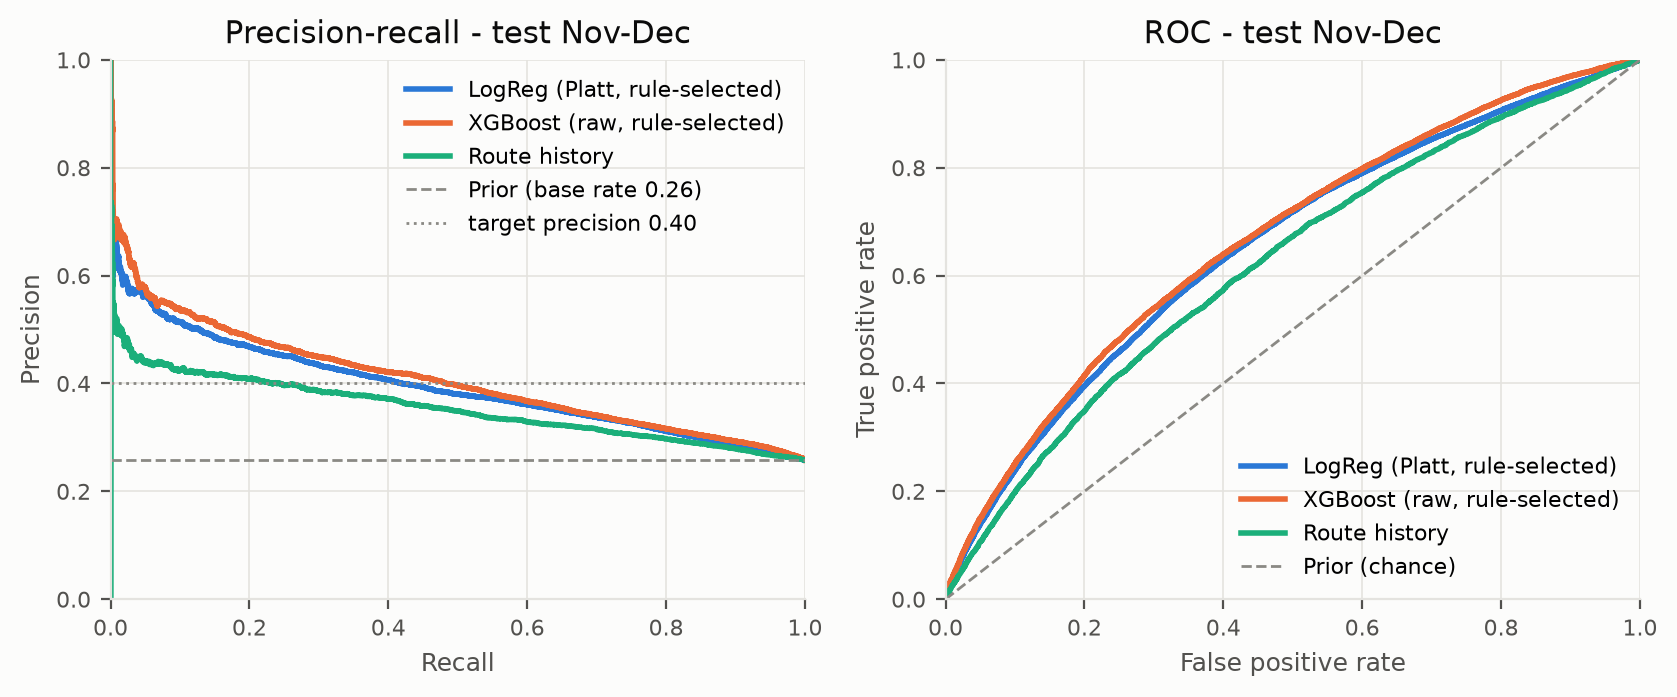
\includegraphics[width=\columnwidth]{pr_roc_test.png}
\caption{Precision--recall and ROC curves on the test window.}
\label{fig:prroc}
\end{figure}

\subsection{Accuracy, precision, recall, F1 and confusion matrix}
These metrics need a yes/no decision, so they are computed at the two operating points declared before testing (Table~\ref{tab:thr}, Fig.~\ref{fig:cm}); no threshold is tuned on the test labels.
\begin{itemize}
\item \textbf{Accuracy is misleading here.} Predicting every flight on time is already 74.2\% accurate on test; this is the prior's frozen-threshold row, which flags nothing because the prior never reaches the precision target. Logistic regression scores 0.740 at the frozen threshold and 0.731 at the daily top 10\%, no better than that trivial rule, although it catches 1{,}972 and 2{,}430 late flights that the trivial rule misses entirely. With one flight in four late, accuracy rewards saying ``on time'', which is why PR-AUC, precision and recall are our main metrics.
\item \textbf{Frozen threshold.} The logistic threshold 0.329 was frozen on Sep--Oct to reach precision 0.40. On test it gives precision 0.491, recall 0.141 and F1 0.220, but it flags 7.4\% of flights instead of 3.8\% on Sep--Oct: a fixed threshold does not fix the workload when the base rate moves. XGBoost's frozen threshold is stricter on test (precision 0.549, recall 0.070).
\item \textbf{Daily top 10\%.} Precision 0.448, recall 0.174 and F1 0.251, the highest F1 in Table~\ref{tab:thr} (XGBoost 0.246, route history 0.201, prior 0.136).
\item \textbf{Most errors are missed delays.} Of the 13{,}946 late test flights, 11{,}974 are predicted on time at the frozen threshold (false negatives), against 2{,}041 false alarms. Much late-running is likely caused by same-day events, such as weather, that evening-before features cannot see, so recall stays low at any precision an operator would accept.
\end{itemize}

\begin{table}[!t]
\caption{Threshold metrics on test at the two operating points declared before testing.}
\label{tab:thr}
\centering\tabsize\setlength{\tabcolsep}{3.5pt}
% generated by scripts/export_report_assets.py from results/ -- do not edit
% needs \usepackage{booktabs}
\begin{tabular}{llrrrr}
\toprule
Model & Policy & Accuracy & Precision & Recall & F1 \\
\midrule
Prior (base rate) & Daily top 10\% & 0.690 & 0.243 & 0.095 & 0.136 \\
Prior (base rate) & Frozen threshold & 0.742 & -- & 0.000 & 0.000 \\
Route history & Daily top 10\% & 0.713 & 0.358 & 0.139 & 0.201 \\
Route history & Frozen threshold & 0.733 & 0.425 & 0.097 & 0.158 \\
LogReg (Platt) & Daily top 10\% & 0.731 & 0.448 & 0.174 & 0.251 \\
LogReg (Platt) & Frozen threshold & 0.740 & 0.491 & 0.141 & 0.220 \\
XGBoost (raw) & Daily top 10\% & 0.729 & 0.438 & 0.171 & 0.246 \\
XGBoost (raw) & Frozen threshold & 0.745 & 0.549 & 0.070 & 0.124 \\
\bottomrule
\end{tabular}

\end{table}

\begin{figure}[!t]
\centering
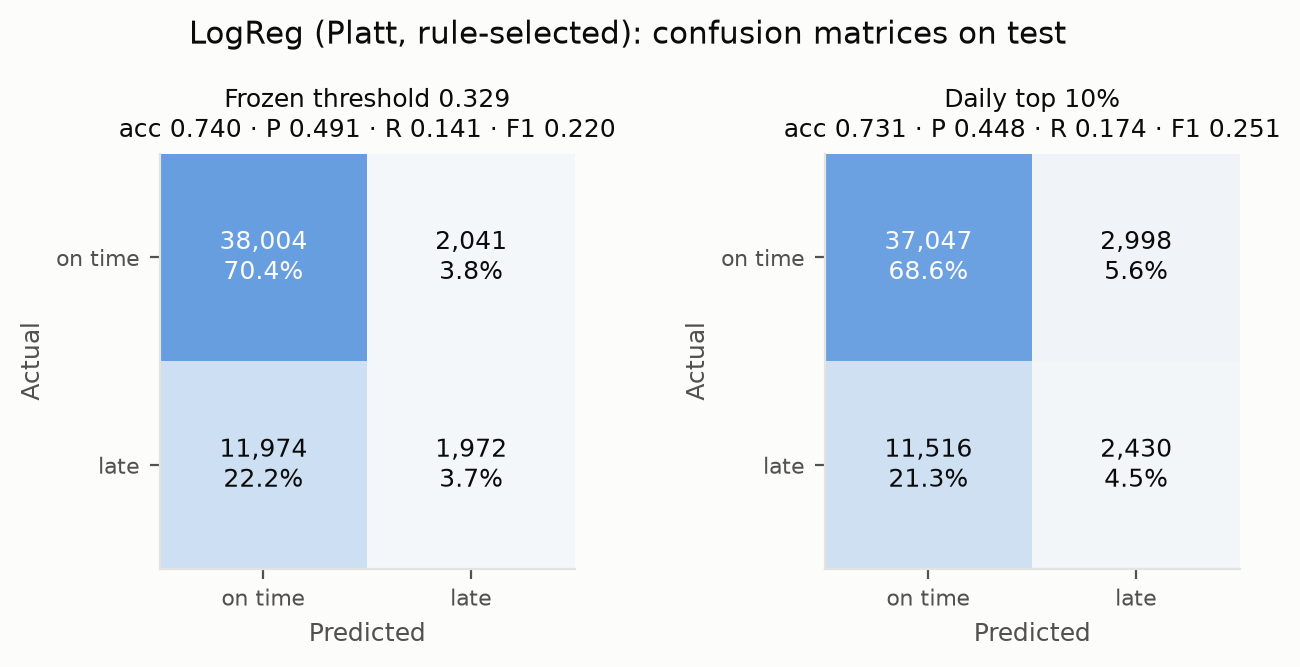
\includegraphics[width=\columnwidth]{confusion_logreg_test.png}
\caption{Confusion matrices of the final model on test (count and share of all flights).}
\label{fig:cm}
\end{figure}

\subsection{Calibration under seasonal shift}
\begin{itemize}
\item \textbf{The static rule fails in December.} Platt scaling fitted on calm Sep--Oct (base rate 15.7\%) scales every risk down. That suits November (ECE 0.022) but not December, whose base rate is 33.5\%: ECE 0.143, and 0.082 over the whole test window (Fig.~\ref{fig:rel}).
\item \textbf{Raw scores look fine only on average.} Raw logistic regression has test ECE 0.019, but 0.056 in November and 0.060 in December: it over-predicts one month and under-predicts the next, and the errors cancel. Fig.~\ref{fig:drift} shows the raw predictions follow the season's shape but compress it.
\item \textbf{Rolling recalibration adapts.} Rolling Platt over 28 days keeps test ECE at 0.027 (November 0.005, December 0.050) for logistic regression and 0.023 for XGBoost. The 28-day window was fixed in advance; 14 and 56 days give 0.021 and 0.051.
\item \textbf{Ranking is unaffected.} Platt scaling is monotone, so both logistic variants rank flights identically and the daily top-10\% policy selects the same flights.
\end{itemize}

\begin{figure}[!t]
\centering
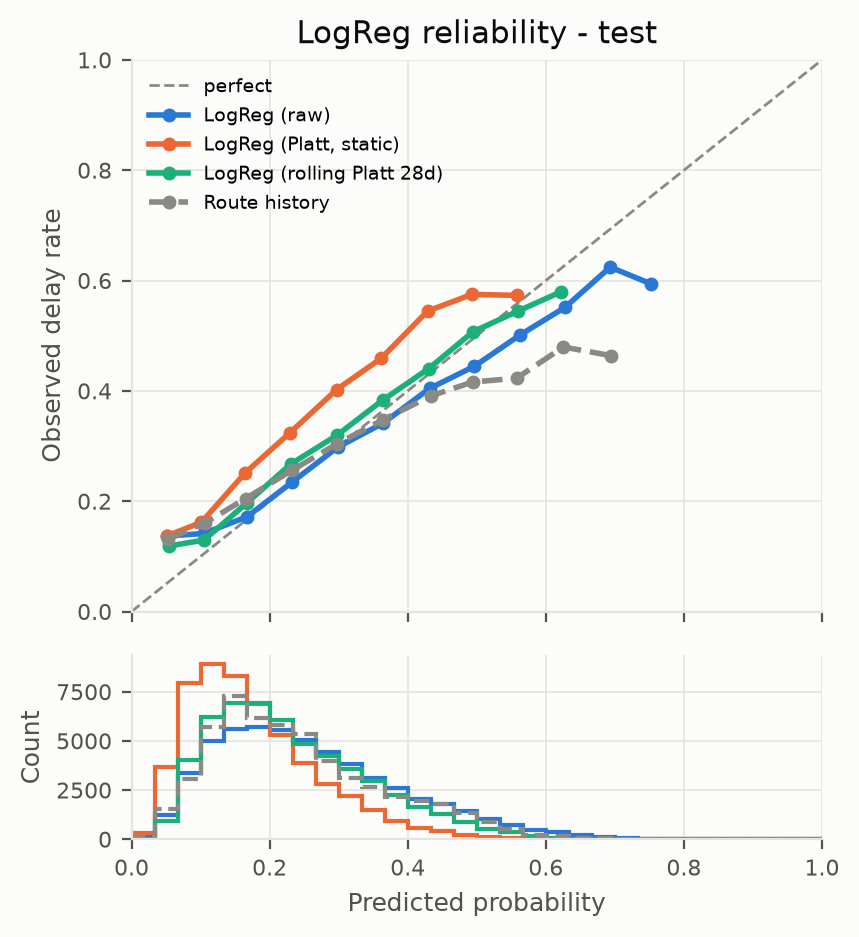
\includegraphics[width=0.82\columnwidth]{reliability_logreg_test.png}
\caption{Reliability of logistic regression on test: raw, static Platt, rolling Platt (28 days) and route history. Bottom: prediction histogram.}
\label{fig:rel}
\end{figure}

\begin{figure}[!t]
\centering
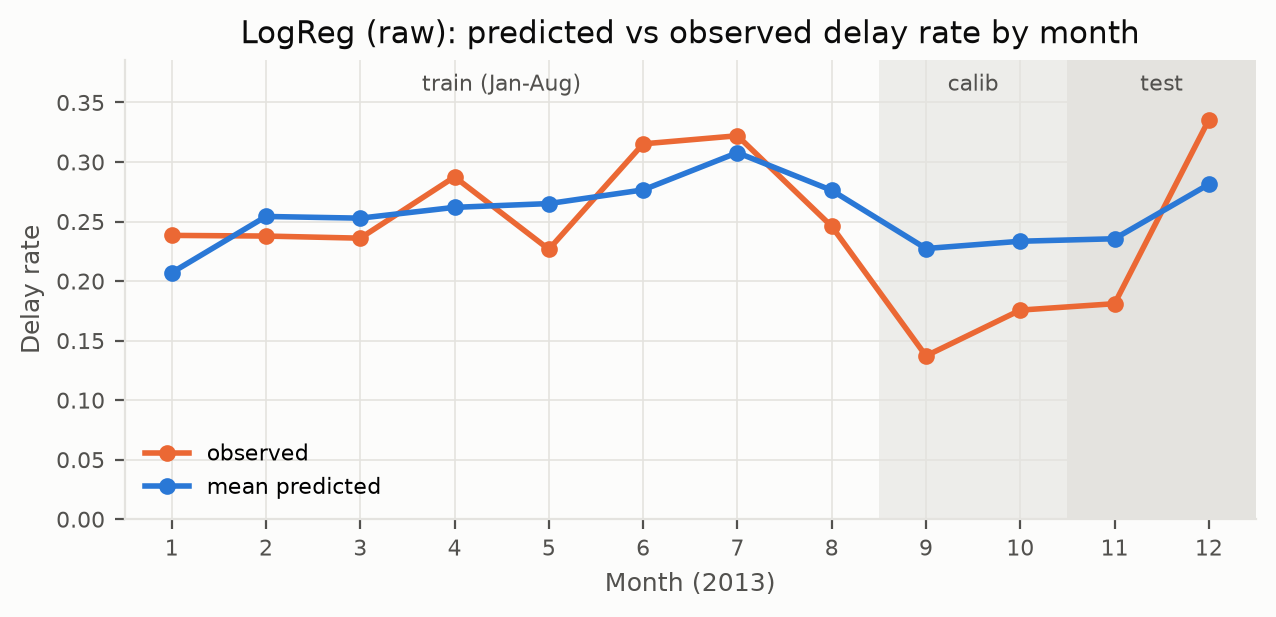
\includegraphics[width=\columnwidth]{monthly_drift_final.png}
\caption{Mean predicted vs observed delay rate by month (raw logistic regression).}
\label{fig:drift}
\end{figure}

\subsection{Which feature groups help?}
\begin{itemize}
\item \textbf{Cross-validation (selection evidence).} Adding groups one at a time to schedule and identifiers raises the CV PR-AUC of logistic regression by 0.021 for congestion (4/4 folds), 0.020 for entity history (4/4) and 0.011 for day history (3/4) (Table~\ref{tab:abl}).
\item \textbf{Test (exploratory).} Only entity history has an interval that excludes zero, for both models (logistic $+0.033$, 95\% CI $[+0.016,+0.050]$).
\item \textbf{Grouped permutation importance} (Sep--Oct, Fig.~\ref{fig:perm}). Each group is shuffled as a whole, so correlated members cannot cover for each other. Shuffling schedule (PR-AUC drop 0.048) or congestion (0.046) hurts logistic regression most, then identifiers (0.038), entity history (0.029) and day history (0.026). This describes the model's sensitivity, not causal effects.
\end{itemize}

\begin{figure}[!t]
\centering
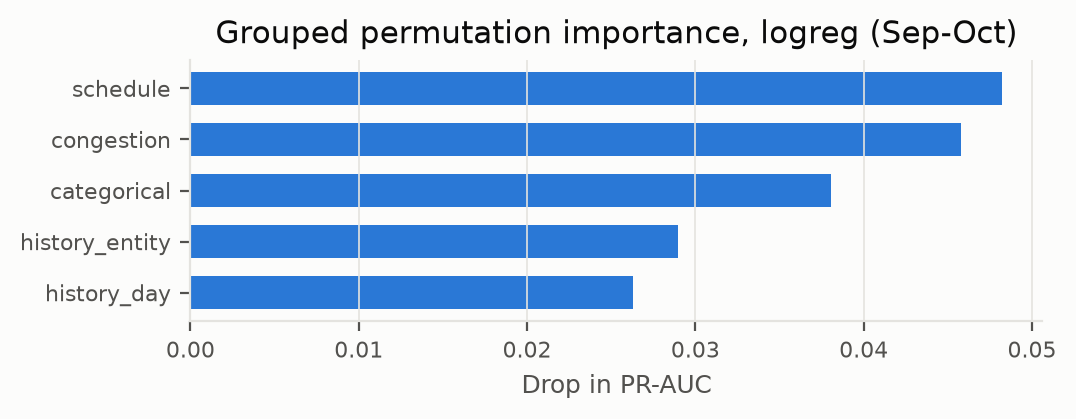
\includegraphics[width=0.92\columnwidth]{perm_importance_groups.png}
\caption{Grouped permutation importance of logistic regression on Sep--Oct.}
\label{fig:perm}
\end{figure}

\begin{table}[!t]
\caption{Feature-group ablation: mean CV gain in PR-AUC (folds improved) and test difference with day-block 95\% CI.}
\label{tab:abl}
\centering\tabsize\setlength{\tabcolsep}{3pt}
% generated by scripts/export_report_assets.py from results/ -- do not edit
% needs \usepackage{booktabs}
\begin{tabular}{llrll}
\toprule
Model & Step & CV gain & Folds & Test diff. [95\% CI] \\
\midrule
LogReg & + congestion & 0.021 & 4/4 & +0.007 [$-$0.010, +0.027] \\
LogReg & + entity history & 0.020 & 4/4 & +0.033 [+0.016, +0.050] \\
LogReg & + day history & 0.011 & 3/4 & +0.009 [$-$0.009, +0.026] \\
XGBoost & + congestion & 0.008 & 3/4 & $-$0.001 [$-$0.014, +0.012] \\
XGBoost & + entity history & 0.007 & 2/4 & +0.048 [+0.026, +0.070] \\
XGBoost & + day history & $-$0.002 & 3/4 & +0.013 [$-$0.020, +0.047] \\
\bottomrule
\end{tabular}

\end{table}

\subsection{Robustness checks}
\begin{itemize}
\item \textbf{Cancelled and diverted flights counted as delayed.} The test base rate rises from 25.8\% to 27.7\%; PR-AUC becomes 0.410 for logistic regression and 0.422 for XGBoost, and the daily top-10\% lift is 1.66 against 0.95 for the prior. Tail-number history features are excluded from this check, because a blank tail number would reveal a cancellation.
\item \textbf{Distribution shift.} The largest single shift is \texttt{days\_to\_holiday} (population stability index 4.8), because Thanksgiving, Christmas and New Year all fall in the test window.
\end{itemize}

%====================================================================
\section{Decision Support: Daily Review Desk}\label{sec:resched}
Each test day, the ranking selects the top $k\%$ of flights as candidates for re-timing or extra buffer, for a desk that can review a fixed share of the roughly 885 daily flights (Table~\ref{tab:resched}).
\begin{itemize}
\item \textbf{Top 10\% (primary policy).} Precision 0.448, recall 0.174, lift 1.73: about 40 delayed flights caught per day, against 32 for route history and 22 for a random ranking.
\item \textbf{Capacity trade-off.} At $k=5\%$ (45 flights a day) precision is 0.474 (lift 1.83); at $k=20\%$ (177 a day) it is 0.406 (lift 1.57) with recall 0.315. Each extra reviewed flight is less likely to be late, so added desk capacity has diminishing returns.
\item \textbf{What this does not show.} It measures ranking quality, not savings: the data contain no cost model and no estimate of how much a schedule change would reduce delay, and weather-driven delays may not be preventable at all.
\end{itemize}

\begin{table}[!t]
\caption{Daily top-$k\%$ review desk on test: flights flagged per day, precision (P), recall (R) and lift of logistic regression (LR), and precision of XGBoost, route history and the random prior ranking.}
\label{tab:resched}
\centering\tabsize\setlength{\tabcolsep}{3.5pt}
% generated by scripts/export_report_assets.py from results/ -- do not edit
% needs \usepackage{booktabs}
\begin{tabular}{llrrrrr}
\toprule
Model & Top share & Flagged/day & Precision & Recall & Lift & Delayed per 100 \\
\midrule
Prior (base rate) & 5\% & 44.705 & 0.251 & 0.049 & 0.971 & 25.083 \\
Prior (base rate) & 10\% & 88.984 & 0.243 & 0.095 & 0.941 & 24.300 \\
Prior (base rate) & 15\% & 133.148 & 0.250 & 0.145 & 0.967 & 24.982 \\
Prior (base rate) & 20\% & 177.393 & 0.252 & 0.195 & 0.974 & 25.164 \\
Route history & 5\% & 44.705 & 0.386 & 0.076 & 1.495 & 38.614 \\
Route history & 10\% & 88.984 & 0.358 & 0.139 & 1.387 & 35.814 \\
Route history & 15\% & 133.148 & 0.346 & 0.201 & 1.339 & 34.597 \\
Route history & 20\% & 177.393 & 0.339 & 0.263 & 1.313 & 33.916 \\
LogReg (Platt, rule-selected) & 5\% & 44.705 & 0.469 & 0.092 & 1.817 & 46.938 \\
LogReg (Platt, rule-selected) & 10\% & 88.984 & 0.444 & 0.173 & 1.720 & 44.436 \\
LogReg (Platt, rule-selected) & 15\% & 133.148 & 0.423 & 0.246 & 1.636 & 42.256 \\
LogReg (Platt, rule-selected) & 20\% & 177.393 & 0.406 & 0.315 & 1.572 & 40.606 \\
XGBoost (raw, rule-selected) & 5\% & 44.705 & 0.464 & 0.091 & 1.797 & 46.425 \\
XGBoost (raw, rule-selected) & 10\% & 88.984 & 0.435 & 0.169 & 1.683 & 43.460 \\
XGBoost (raw, rule-selected) & 15\% & 133.148 & 0.416 & 0.242 & 1.611 & 41.603 \\
XGBoost (raw, rule-selected) & 20\% & 177.393 & 0.400 & 0.310 & 1.548 & 39.996 \\
\bottomrule
\end{tabular}

\end{table}

%====================================================================
\section{Discussion and Limitations}\label{sec:discussion}
\begin{itemize}
\item \textbf{What the evidence supports.} Day-ahead risk ranking is useful: the top tenth of each day is 1.73 times more often late than average, clearly above the route heuristic (1.39). With these engineered features, the extra flexibility of XGBoost gives no clear gain: the two models are within noise of each other.
\item \textbf{Calibration needs monitoring.} A calibrator fitted once fails when the season changes; recalibrating on recent \emph{known} outcomes worked here, but is not guaranteed to work under every shift.
\item \textbf{Threats to validity.} The test window was seen during development (Sec.~\ref{sec:protocol}). One year and three airports observe each season once, so cross-year generalisation is untested. Four CV folds cannot separate models that differ by a few thousandths.
\item \textbf{Limitations.} No weather, by design: observed weather for day $D$ is not available at 20:00 on $D-1$, and archived forecasts were not available to us. Only NYC departures are visible, so delay propagation along an aircraft's full rotation is not modelled. Tail-number assignments are assumed known the evening before. The what-if rescheduling simulation requested by the project brief is not yet done; Sec.~\ref{sec:resched} supplies only its candidate-selection step.
\end{itemize}

%====================================================================
\section{Conclusion}\label{sec:conclusion}
A decision clock, enforced by tests rather than by convention, is the backbone of an honest day-ahead model; a test that cancels flights exactly as the raw data records them exposed a leak in two otherwise plausible features. Under that clock, a regularised logistic regression on shrunk history rates matches XGBoost and lifts the precision of a daily review desk to 1.73 times the base rate. Probabilities need more care than rankings: a static calibrator broke in December, and a causal rolling recalibration repaired it.

\textbf{Future work.} An embedding-based MLP for airline and airport interactions (Phase~2), weather forecasts archived before the clock, several years of data, and a what-if rescheduling simulation with explicit intervention assumptions.

\textbf{Code and data.} Code, notebooks, saved results and detailed per-stage notes: \url{https://github.com/nipun1803/AeroCast-AI}. All randomness is seeded (42).

\bibliographystyle{IEEEtran}
\bibliography{references}

\end{document}
